\documentclass[lang=cn,12pt, scheme=chinese]{elegantbook}


\usepackage{amsmath}
\usepackage{slashed}
\usepackage{mathtools}
\usepackage{cancel}
\usepackage{wrapfig}
\usepackage{tikz}
\usetikzlibrary{positioning, shapes.geometric, arrows.meta}
\usepackage{ulem}
%\usepackage{CJKulem}
\usepackage{xeCJK}
\usepackage{CJKfntef}
\usepackage{indentfirst}


\title{课程学习笔记}
% \subtitle{Classic Elegant\LaTeX{} Template}

\author{S.Y. Chen}
\bioinfo{单位}{Southwest University}
\bioinfo{时间}{\today}
% \institute{Southwest University}
% \date{\today}
% \version{3.11}
% \bioinfo{Bio}{Information}

\extrainfo{Victory won\rq t come to us unless we go to it. }

\logo{logo-blue.png}
\cover{cover.jpg}

\begin{document}

\maketitle

\frontmatter
\tableofcontents

\mainmatter

%%%%%%%%%%%%%%%%%%%%%%%%%%%%%%%%%%%%%%%%%%%%%%%%
\chapter{液滴模型}
%%%%%%%%%%%%%%%%%%%%%%%%%%%%%%%%%%%%%%%%%%%%%%%%%%%%%%%%%%%%%%%%%%%%%%%%%%%%%%%%%%
\section{引言}
\textbf{液滴模型(LDM)提出的依据:}
\begin{enumerate}
	\item 原子核的不可压缩性:一般的,我们认为原子核无法的压缩性极低,且其体积不随其形状的改变而发生变化;
	\item 原子核具有明确的表面(well defined surface);
	\item 原子核中核力的\textcolor{red}{\underline{饱和性质:}}原子核中的一个核子仅与有限个核子发生相互作用。
\end{enumerate}

基于上面原子核的性质,人们提出了所谓的液滴模型,将原子核当成一个均匀带电的、不可压缩的、体积不变的液滴。从严格意义上来讲,这与真实的原子核情况是不相符的:原子核还具有结团(cluster)现象,表现为质量数等于4的核较为稳定;此外,在经典液滴中,两粒子的平均距离由粒子间作用力的极小值给出,大约为0.7fm,但是真实原子核应该是一个量子流体,其中的粒子间平均距离约为2.4fm,这是因为核子是满足费米统计(Fermi statistics)的,此时,泡利原理(Pauli principle)会阻止核子间距离过于接近,从而切掉了大部分两体力,导致核子间距离变大;在一个量子流体中是很少发生散射的,而在经典液滴中则以散射为主要反应。

\textbf{原子核的结合能:}对于一个包含$A$个粒子的系统,其结合能若只由两体力提供,那么它的总结合能$B(N,Z)$与粒子所构成的两体相互作用的组合数成正比关系,即有如下关系成立:
\begin{equation*}
	B(N, Z) \propto
	\begin{pmatrix}
		2	\\
		A
	\end{pmatrix}
	= \frac{1}{2} A(A-1)
\end{equation*} 
上述关系的例子可参考原子中的电子结合能。按上所述,原子核的总结合能$B(N,Z)$应随质量数的增大而增大,而且其\underline{\textcolor{red}{每核子的结合能}}(或称\underline{\textcolor{red}{比结合能}})应随质量数呈线性递增的关系,但实验发现对于质量数$A > 12$的原子核,其比结合能会大致处在某一常数附近
\begin{equation}
	\frac{B(N, Z)}{A} \simeq -8.5 [\text{ MeV/nucleon }]  \label{eq_specific_binding_energy}
\end{equation} 
原子核中结合能的行为可由核力的饱和性质进行解释。而这最后可归因到核力的短程性以及泡利原理与不确定性原理的结合。
\begin{note}
	核力是短程力的表现:核力的作用范围为$< 1.5 \times 10^{-15} {\rm m}$,在大于$0.8 \times 10^{-15} {\rm m}$ 时表现为吸引力,而且随着距离的增大而减小,当两核子距离$> 1.5 \times 10^{-15} {\rm m}$时核力会迅速降低并消失;两核子距离$ < 0.8 \times 10^{-15} {\rm m}$时,核力表现为排斥力,且随距离的减小而增大。
\end{note}

\textbf{原子核半径:}若将原子核描述为一个密度为常数并且具有sharp表面的球体,那么其半径可取经验公式
\begin{equation}
	R = r_0 A^{1/3}	\label{eq_nuclear_radius}
\end{equation} 
参数$r_0$一般取经验值$r_0 = 1.2 {\rm fm}$。

\textbf{原子核结合能的半经验公式:}根据液滴模型,C.F. Weizaker提出了原子核结合能的半经验公式:
\begin{equation}
	B(N, Z) = a_V A + a_S A^{2/3} + a_C \frac{Z^2}{A^{1/3}} + a_I \frac{(N-Z)^2}{A} - \delta(A)	\label{eq_semi-empirical_mass_formula}
\end{equation} 
其中拟合参数为
\begin{equation}
    \begin{aligned}
		a_V = -15.68; \quad a_S = 18.56; \quad a_C = 0.717; \quad a_I = 28.1	\quad	[MeV]	\\
		\delta(A) = \left\{ \begin{array}{cc}
				34 \cdot A^{-3/4} & \text{ for even-even } \\
				0 & \text{ for even-odd }	\\
				-34 \cdot A^{-3/4} & \text{ for odd-odd }
		\end{array}\right\} \text{nuclei}
    \end{aligned}
    	\label{eq_semi-empirical_mass_formula_fit}
\end{equation} 
式\eqref{eq_semi-empirical_mass_formula_fit}等号右边逐项的物理解释如下:
\begin{enumerate}
	\item 第一项:体积能项,因为$ A \propto R^3$,对应于球形的体积公式;
	\item 第二项:表面能项,因为$ A^{2/3} \propto R^2$,对应于球形面积公式;
	\item 第三项:库伦能项,表示质子间的库伦排斥项。库伦能正比于原子核中的质子对数量($\propto Z^2$),并与半径称反比。
	\item 第四项:对称能项,若没有泡利原理,由于质子间存在库仑斥力,因此原子核更倾向于仅包含中子的情况;
	\item 第五项:对能项,考虑到偶偶核、偶奇核、奇奇核的质量差等因素。
\end{enumerate}
得到结合能公式后的拟合图像如下图所示


\section{形变参数}
\textbf{形变原子核半径:}原子核的形状可体现在其表面上某一点到原点的距离,也就是形变核核中从原点到表面的半径矢量
\begin{equation}
	R = R(\theta, \phi) = R_0 ( 1 + \alpha_{00} + \sum_{\lambda = 1}^{\infty} \sum_{\mu = -\lambda}^{\lambda}\alpha^{*}_{\lambda\mu} Y_{\lambda\mu}(\theta, \phi) )	\label{eq_deform_radius}
\end{equation} 
其中$R_0$表示相同体积的球形核半径。此公式并非唯一描述该半径的公式,但却是最常用的。







\chapter{原子核平均场和多核子组态}

%%%%%%%%%%%%%%%%%%%%%%%%%%%%%%%%%%%%%%%%%
\section{原子核平均场}
\paragraph*{准粒子} 准粒子一般用来作为粒子近似。准粒子系统可以当成无相互作用的准粒子进行处理。
\paragraph*{平均场近似} 我们通常将强相互作用的粒子系统转换到弱相互作用的准粒子系统来处理多体问题。以下将讨论所谓的平均场(或Hartree-Fock)准粒子。在像原子核这样的多体系统中,核子-核子相互作用可忽略掉三体及以上的多体相互作用,最高写成两体相互作用的形式,其哈密顿量由动能项和势能项组成:
\begin{equation}
	H = T + V = \sum_{i = 1}^{A} t(\boldsymbol{r}_i) + \sum_{i, j = 1; i < j}^{A} v(\boldsymbol{r}_i, \boldsymbol{r}_j) =  \sum_{i = 1}^{A} \frac{-\hbar^2}{2m_N}\nabla_i^2 + \sum_{i, j = 1; i < j}^{A} v(\boldsymbol{r}_i, \boldsymbol{r}_j) 
\end{equation}

\chapter{原子核平均场及多核子组态}

\section{原子核平均场}
\paragraph*{平均场近似:}
\begin{enumerate}
	\item 质量数$A$,质子数$Z$,中子数$N$,满足$A=N+Z$;
	\item 核子间有强相互作用(核力),特别的,质子直接按
	\item 把核子当成没有内部结构的点粒子;
\end{enumerate}

\paragraph*{原子核集体波函数$\Psi_0$的理解:}在\uline{\textsl{Hartree}}方法中,集体波函数
只表现为单粒子态的直积形式,如下
\begin{equation}
	\Psi_0(\bm{r}_1,\ \bm{r}_2,\ \bm{r}_3,\cdots,\ \bm{r}_A) = \prod_{i=1}^{A} 
    \phi_{\alpha_i}(\bm{r}_i)
\end{equation} 
在\uline{\textsl{Hartree-Fock}}方法中,集体波函数表现为有个单粒子直积形式的混合,且具有反
对称性质,如下
\begin{equation}
    \begin{aligned}
		\Psi_0(\bm{r}_1, \bm{r}_2, \bm{r}_3, \cdots, \bm{r}_A) ={}& \mathcal{A}\left[ 
        \prod_{i=1}^{A} \phi_{\alpha_i}(\bm{r}_i) \right]	\\
		={}& 
		\begin{vmatrix}
			\phi_1(\bm{r}_1)	&	\phi_1(\bm{r}_2)	&	\phi_1(\bm{r}_3)	&	\cdots	&	\phi_1(\bm{r}_A)	\\
			\phi_2(\bm{r}_1)	&	\phi_2(\bm{r}_2)	&	\phi_2(\bm{r}_3)	&	\cdots	&	\phi_2(\bm{r}_A)	\\
			\phi_3(\bm{r}_1)	&	\phi_3(\bm{r}_2)	&	\phi_3(\bm{r}_3)	&	\cdots	&	\phi_3(\bm{r}_A)	\\
			\vdots				&	\vdots				&	\vdots				&	\ddots	&	\vdots				\\
			\phi_A(\bm{r}_1)	&	\phi_A(\bm{r}_2)	&	\phi_A(\bm{r}_3)	&	\cdots	&	\phi_A(\bm{r}_A)	\\
		\end{vmatrix}
    \end{aligned}
\end{equation} 
	其中,$\mathcal{A}$为反对称化算符,并且包含了归一化系数;$\bm{r}_1,\ \bm{r}_2,\ \cdots,
    \ \bm{r}_A$表示粒子$1,\ 2,\ \cdots,\ A$的坐标;$\phi_1,\ \phi_2,\ \cdots,\ \phi_A$表
    示有那么多个能级,也就是粒子可能占据的能级。我们现在考虑三粒子体系的情况,三个粒子占
    据三个能级,在\textsl{Hartree-Fock}方法中,其集体波函数可表示为
\begin{equation}
    \begin{aligned}
		\Psi_0(\bm{r}_1, \bm{r}_2, \bm{r}_3) ={}& \mathcal{A}\left[ \prod_{i=1}^{3} 
        \phi_{\alpha_i}(\bm{r}_i) \right]	\\
		={}& \frac{1}{\sqrt{6}} 
		\begin{vmatrix}
			\phi_1(\bm{r}_1)	&	\phi_1(\bm{r}_2)	&	\phi_1(\bm{r}_3)	\\
			\phi_2(\bm{r}_1)	&	\phi_2(\bm{r}_2)	&	\phi_2(\bm{r}_3)	\\
			\phi_3(\bm{r}_1)	&	\phi_3(\bm{r}_2)	&	\phi_3(\bm{r}_3)	\\
		\end{vmatrix}	\\
		={}& \phi_1(\bm{r}_1)\phi_2(\bm{r}_2)\phi_3(\bm{r}_3) + \phi_1(\bm{r}_2)\phi_2(\bm{r}_3)\phi_3(\bm{r}_1) + \phi_1(\bm{r}_3)\phi_2(\bm{r}_1)\phi_3(\bm{r}_2) \\
		&- \phi_1(\bm{r}_3)\phi_2(\bm{r}_2)\phi_3(\bm{r}_1) - \phi_1(\bm{r}_2)\phi_2(\bm{r}_1)\phi_3(\bm{r}_3) - \phi_1(\bm{r}_1)\phi_2(\bm{r}_3)\phi_3(\bm{r}_2) 
    \end{aligned}
\end{equation} 
现在我们考察上式第二个等号的左边第一项,$\phi_1(\bm{r}_1)\phi_2(\bm{r}_2)\phi_3(\bm{r}_3)$表示粒子$1$处于能级$\phi_1$、位置在$\bm{r}_1$,且粒子$2$处于能级$\phi_2$、位置在$\bm{r}_2$,同时粒子$3$处于能级$\phi_3$、位置在$\bm{r}_3$的概率;后面几项类同。事实上,由于全同粒子的不可区分性,我们根本无法辨别粒子$1$、$2$、$3$,因此我们无法判断具体某一个态上的粒子具体是$1$、$2$、$3$中的哪一个,所以我们需要把各种情况考虑进来,同时考虑费米子的交换反对称性应加上对应的相位,上式最后一个等号右边的排列情况构成了如图\ref{fig:three-body-wv}所示:
\begin{figure}[htbp]
	\centering
	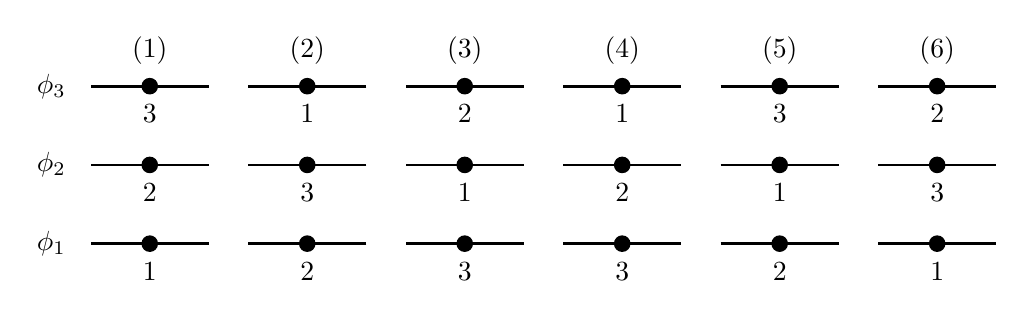
\begin{tikzpicture}
		\node at (-6.25, 2) {$\phi_3$};
		\node at (-6.25, 1) {$\phi_2$};
		\node at (-6.25, 0) {$\phi_1$};

		\node at (-5, 2.45) {(1)};
		\draw[line width=1pt] (-4.25, 2) -- (-5.75, 2);
		\draw[line width=1pt] (-4.25, 1) -- (-5.75, 1);
		\draw[line width=1pt] (-4.25, 0) -- (-5.75, 0);
		\fill (-5, 0)circle(3pt) (-5, 1)circle(3pt) (-5, 2)circle(3pt);
		\node at (-5, -0.35) {$1$};
		\node at (-5,  0.65) {$2$};
		\node at (-5,  1.65) {$3$};

		\node at (-3, 2.45) {(2)};
		\draw[line width=1pt] (-2.25, 2) -- (-3.75, 2);
		\draw[line width=1pt] (-2.25, 1) -- (-3.75, 1);
		\draw[line width=1pt] (-2.25, 0) -- (-3.75, 0);
		\fill (-3, 0)circle(3pt) (-3, 1)circle(3pt) (-3, 2)circle(3pt);
		\node at (-3, -0.35) {$2$};
		\node at (-3,  0.65) {$3$};
		\node at (-3,  1.65) {$1$};

		\node at (-1, 2.45) {(3)};
		\draw[line width=1pt] (-0.25, 2) -- (-1.75, 2);
		\draw[line width=1pt] (-0.25, 1) -- (-1.75, 1);
		\draw[line width=1pt] (-0.25, 0) -- (-1.75, 0);
		\fill (-1, 0)circle(3pt) (-1, 1)circle(3pt) (-1, 2)circle(3pt);
		\node at (-1, -0.35) {$3$};
		\node at (-1,  0.65) {$1$};
		\node at (-1,  1.65) {$2$};

		\node at (1, 2.45) {(4)};
		\draw[line width=1pt] (0.25, 2) -- (1.75, 2);
		\draw[line width=1pt] (0.25, 1) -- (1.75, 1);
		\draw[line width=1pt] (0.25, 0) -- (1.75, 0);
		\fill (1, 0)circle(3pt) (1, 1)circle(3pt) (1, 2)circle(3pt);
		\node at (1, -0.35) {$3$};
		\node at (1,  0.65) {$2$};
		\node at (1,  1.65) {$1$};

		\node at (3, 2.45) {(5)};
		\draw[line width=1pt] (2.25, 2) -- (3.75, 2);
		\draw[line width=1pt] (2.25, 1) -- (3.75, 1);
		\draw[line width=1pt] (2.25, 0) -- (3.75, 0);
		\fill (3, 0)circle(3pt) (3, 1)circle(3pt) (3, 2)circle(3pt);
		\node at (3, -0.35) {$2$};
		\node at (3,  0.65) {$1$};
		\node at (3,  1.65) {$3$};

		\node at (5, 2.45) {(6)};
		\draw[line width=1pt] (4.25, 2) -- (5.75, 2);
		\draw[line width=1pt] (4.25, 1) -- (5.75, 1);
		\draw[line width=1pt] (4.25, 0) -- (5.75, 0);
		\fill (5, 0)circle(3pt) (5, 1)circle(3pt) (5, 2)circle(3pt);
		\node at (5, -0.35) {$1$};
		\node at (5,  0.65) {$3$};
		\node at (5,  1.65) {$2$};
	\end{tikzpicture}	
	\caption{三粒子填充三条能级的体系集体波函数情况}
	\label{fig:three-body-wv}
\end{figure}

\paragraph*{平均场的迭代求解:}
平均场下的\textsl{Hartree(-Fock)}方程如下:
\begin{equation}
    \begin{aligned}
        \frac{-\hbar^{2}}{2m_N} \nabla^{2} \phi_{\alpha}(\bm{r}) + V_{H(F)}\left(
        \{\phi_{i}(\bm{r})\}\right) = \varepsilon_{\alpha}\phi_{\alpha}(\bm{r}) \\ 
        i = 1, 2, \cdots, A, \quad \alpha = 1, 2, \cdots, \infty
    \end{aligned}
    \label{eq:Hartree-Fock}
\end{equation}
上式与薛定谔方程唯一不同就是势能变成了关于波函数的非线性函数,
\begin{equation*} V(\bm{r}) \Longrightarrow V_{H(F)}(\{\phi_{i}(\bm{r})\})
\end{equation*}
式\eqref{eq:Hartree-Fock}为非线性方程组,一般用迭代的方法求解。我们先猜测得到一组试探
波函数${\phi_i^0(\bm{r})}_{i=1}^{A}$,然后我们根据势能与波函数的关系得到初始势场
$V_{H(F)}^{0}$;完成上述步骤后,我们将试探波函数和初始势场带入式\eqref{eq:Hartree-Fock},
求解得到一组新的波函数${\phi_{\alpha}^0(\bm{r})}_{\alpha=1}^{A}$和本征值$\varepsilon_{\alpha}^{(1)}$,
通过这组新的波函数,我们可以再次生成一个新的势场$V_{H(F)}^{(1)}$;将生成的新势场和新波函数
再次代入式\eqref{eq:Hartree-Fock},可得到更新一组的本征波函数和本征能量。通过比较某次迭代
前后的波函数间的误差小于某一给定值来确定波函数合理
\begin{equation}
    \parallel \phi_{\alpha}^{(n-1)} - \phi_{\alpha}^{(n)} \parallel < \text{preset limit}
    \label{eq:iter-error}
\end{equation}
其中,$\parallel \cdots \parallel$表示波函数的模。

\uline{关于平均势场和初始波函数形式的选取}:上述平均场方程中,势能具体形式为
\begin{equation}
    V_{H(F)}\left( \left\{ \phi_i(\bm{r}) \right\} \right) = \sum_{i \neq j} \int 
    \phi_i^{\star}(\bm{r}_i^{\prime}) V_{ij}(\bm{r}_i^{\prime}, \bm{r}_j) \phi_{i}(\bm{r}_i^{\prime})
    \,d\bm{r}_i^{\prime}
    \label{eq:mean-field}
\end{equation}
为寻找到一组合适的平均场,试探波函数可以选取一组零级近似,如费米气体模型单粒子波函数:
\begin{equation}
    \phi_i = \sqrt{V^{-1}} \exp{(i \bm{k}_i \cdot \bm{r}_i)}
    \label{eq:fermi-gas-eigen}
\end{equation}
其中,$V$表示原子核的体积。对于二体势$V_{ij}$,可以选用Skyrme力(见下式)或其它形式的两体力
\begin{equation}
    V_{skyrme} = \sum_{i<j} v(i, j) + \sum_{i<j<k} v(i, j, k)
    \label{eq:skyrme-forc}
\end{equation}
其中,两体力部分为
\begin{equation}
    \begin{aligned}
        v(1, 2) =& t_0 (1 + x_0 P_{\sigma})\delta(\bm{r}_1 - \bm{r}_2) \\
            & + t_1\left[ \delta(\bm{r}_1 - \bm{r}_2) \bm{k}^{2}
              + \bm{k}^{\prime 2}\delta(\bm{r}_1 - \bm{r}_2)\right] / 2 \\
            & + t_2\bm{k}^{\prime} \cdot \delta(\bm{r}_1 - \bm{r}_2) \bm{k} \\
            & + {\rm i} W_0(\bm{\sigma}_1 + \bm{\sigma}_2)\cdot \left[ 
            \bm{k}^{\prime} \times \delta\left( \bm{r}_1 - \bm{r}_2 \right) \bm{k}\right]
    \end{aligned}
    \label{eq:skyrme-tow-body-forc}
\end{equation}
三体部分为
\begin{equation}
    v(1, 2, 3) = t_3 \delta(\bm{r}_1 - \bm{r}_2) \delta(\bm{r}_2 - \bm{r}_3)
    \label{eq:skyrm-three-body-forc}
\end{equation}
式中,$\bm{k} = \bm{p}/\hbar = (\nabla_{1} - \nabla_{2}) / (2{\rm i})$是向右作用的相对动量
算符,$\bm{k}^{\prime} = \bm{p}/\hbar = (\nabla_{2} - \nabla_{1}) / (2{\rm i})$是向左相对
动量算符;$P_{\sigma} = (1 + \bm{\sigma}_1 \cdot \bm{\sigma}_2) / 2$是自旋交换算符。上式
Skyrme力有6个可调参数$t_0$、$t_1$、$t_2$、$t_3$、$x_0$和$W_0$。

\section{Woods-Saxon波函数用球谐振子基展开}
单核子薛定谔方程中的哈密顿量为:
\begin{equation}
	\begin{aligned}
		h =& \frac{-\hbar^2}{2 m_{N}} \nabla^2 + v(r) + v_{LS}(r) \boldsymbol{L\cdot S}	\\
		=& \frac{-\hbar^2}{2 m_{N}}\left(\nabla^2_{r} - \frac{\boldsymbol{L}/\hbar^2}{r^2} + v_{WS}(r) + v_{C}(r) + v_{LS}(r)\boldsymbol{L\cdot S}\right)
	\end{aligned}
\end{equation} 
其中,径向偏分取一般形式
\begin{equation}
	\nabla^2_{r} \equiv \frac{1}{r^2} \frac{d}{dr} \left(r^2 \frac{d}{dr}\right)
\end{equation}
$v_{WS}$是Woods-Saxon势,$v_{C}(r)$为库伦势,原子核半径内取均匀带电的球静态库伦势,可得方程如下
\begin{equation}
	v_{C} = \frac{Ze^2}{4\pi\epsilon_0}
\end{equation} 

\section{Woods-Saxon哈密顿量的对角化}
得到球谐振子波函数后,可将这些波函数作为基矢展开构成Woods-Saxon势下的原子核波函数。谐振子展开的Woods-Saxon径向哈密顿量矩阵元为
\begin{equation}
    \begin{aligned}
		\langle \nu^{\prime} | h_{lj}(r) | \nu\rangle =&\int_{0}^{\infty} r^2 \,dr g_{\nu^{\prime} l}(r) g_{\nu l}(r) \left[ \frac{\hbar^2}{2m_N} \left(\frac{4n + 2l + 3}{b^2} - \frac{r^2}{b^4}\right) \right. \\
		&+ \left. v_{WS}(r) + v_{C}(r) + \frac{1}{2}\left[j(j+1) - l(l+1) - \frac{3}{4}\hbar^2 v_{LS}(r)\right] \right]
    \end{aligned}
\end{equation}
这样,整个矩阵就可以写成如下形式
\begin{equation}
	\begin{bmatrix}
		\langle 0 | h_{lj}(r) | 0 \rangle & \langle 0 | h_{lj}(r) | 1 \rangle & \cdots	& \cdots	\\
		\langle 1 | h_{lj}(r) | 0 \rangle & \langle 1 | h_{lj}(r) | 1 \rangle & \cdots	& \cdots	\\
		\vdots	&	\vdots	& \ddots
	\end{bmatrix}
\end{equation}
这样,当我们对角化该矩阵后就可以知道此径向哈密顿量在谐振子基上的能量,通过比例关系就可以知道对应谐振子基上的系数$A_{\nu}^{(nlj)}$。



\chapter{占据数表象}

\section{多粒子态表象}
\paragraph*{$N$粒子系统的基矢:}以某一中原子核组态$|\alpha_1\ \alpha_2 \cdots \alpha_N\rangle$

\appendix
\chapter{变分原理及其应用}

%%%%%%%%%%%%%%%%%%%%%%%%%%%%%%
\section{变分原理}
在二维直角坐标中有两个定点$(x_1,\ y_1)$、$(x_2,\ y_2)$,连接这两点的任意一条曲线为$y = y(x)$,其满足边界条件如下:
\begin{equation}
    y(x_1) = y_1, \quad y(x_2) = y_2
\end{equation} 
现在,我们定义一个新的函数$f$,它是关于$y$和$y^{\prime}$($y$的一阶导数)的函数,形式为$f = f(y, y^{\prime})$,我们对其做关于$x$的定积分,如下
\begin{equation}
	I = \int_{x_1}^{x_2} f(y, y^{\prime}) \, dx	\label{eq:variation-simple}
\end{equation} 
这样,当$y$变化时,定积分$I$也会随之改变,这样,我们期望能找到某一个$y$,使$I$有极值(极大或极小)。

我们回顾一下以往的极值问题,对于某一个函数$y=y(x)$,我们变化自变量$x$,通过对比不同$x$处的函数值$y$来找到极值;现在我们来看式\eqref{eq:variation-simple},它的积分变量是$x$,且积分区间固定,我们无法通过改变$x$来改变$I$的值,但是被积函数$f$是关于$y$和$y^{\prime}$的函数,它的形式并不确定,因此,针对式$\eqref{eq:variation-simple}$的变分问题,我们考察的是:取不同形式的$y(x)$,使积分$I$有极值。\CJKunderdot{\textcolor{red}{我们习惯上把$I$称作$y(x)$的泛函}}【也就是函数的函数,$f$是$y$的函数,$I$是$f$的函数;或者$y$是$x$的函数($x$变化范围,例如从$x=1$变为$x=2$),$I$是$y$的函数($y$变换形式,如$y=x$变为$y=x^2$)】。由于取的是$I$的极值,因此当我们对$y(x)$做微小的变化是,$I$在一级近似下应该不变(也就是$I$关于$y$的一阶导为0)。$\delta y$是$y$的无穷小变化,习惯上把\CJKunderdot{\textcolor{red}{$\delta y$称为$y$的变分}}。

当我们变化$\delta y$时,$f$的变化为
\begin{equation}
	\delta f = \frac{\partial f}{\partial y} \delta y + \frac{\partial f}{\partial y^{\prime}} \delta y^{\prime}
\end{equation} 
$I$相应的变化为
\begin{equation}
	\delta I = \int_{x_1}^{x_2} \delta f \, dx = \int_{x_1}^{x_2} \left[  \frac{\partial f}{\partial y} \delta y + \frac{\partial f}{\partial y^{\prime}} \delta y^{\prime} \right] \, dx	\label{eq:variation}
\end{equation} 
方括号第二项用分部积分方法
\begin{equation}
	\begin{aligned}
		\int_{x_1}^{x_2} \frac{\partial f}{\partial y^{\prime}} \delta y^{\prime}\, dx =&{} \int_{x_1}^{x_2} \frac{\partial f}{\partial y^{\prime}} \left( \frac{d (\delta y)}{dx} \right) \, dx = \int_{x_1}^{x_2} \frac{\partial f}{\partial y^{\prime}} \, d (\delta y)	\\
		=&{} \left. \left( \frac{\partial f}{\partial y^{\prime}} \delta y \right) \right|_{x_1}^{x_2} - \int_{x_1}^{x_2} \delta y \frac{d}{dx}\left( \frac{\partial f}{\partial y^{\prime}} \right) \, dx
	\end{aligned}
\end{equation} 
考虑到边界是固定的,也就是在$x=x_1$和$x=x_2$出函数值$y(x_1)$和$y(x_2)$保持不变,因此我们有$\delta y(x_1) = \delta y(x_2) = 0$,上式最后一个等号右边第一项为0,即
\begin{equation}
	\left[ \frac{\partial f}{\partial y^{\prime}} \delta y \right]_{x_1}^{x_2} = 0
\end{equation}
将以上两式带回到式\eqref{eq:variation},得到
\begin{equation}
	\delta I = \int_{x_1}^{x_2} \left[ \frac{\partial f}{\partial y} - \frac{d}{dx}\left( \frac{\partial f}{\partial y^{\prime}} \right) \right] \, dx
\end{equation} 
若要求$I$有极值,则$\delta I = 0$,那么有下式成立
\begin{equation}
    \frac{\partial f}{\partial y} - \frac{d}{dx}\left( \frac{\partial f}{\partial y^{\prime}} \right) = 0
\end{equation} 
上式则是\textcolor{red}{Euler-Lagrange方程}。

\section{变分原理与Schr\"{o}dinger方程}
我们可以从变分原理出发,推导出Schr\"{o}dinger方程。

体系的Hamilton量为$\hat{H}$,




\end{document}
